\chapter{Verteilungssicht}
Das System besteht aus einem Server, einem oder mehreren Client-Geräten als Display und einem oder mehreren Fernbedienungen. Wie diese miteinander verbunden sind ist in dem Diagramm in Abbildung \ref{fig:verteilusgssicht} dargestellt.\\
\\
\begin{minipage}{\textwidth} 
	\centering
	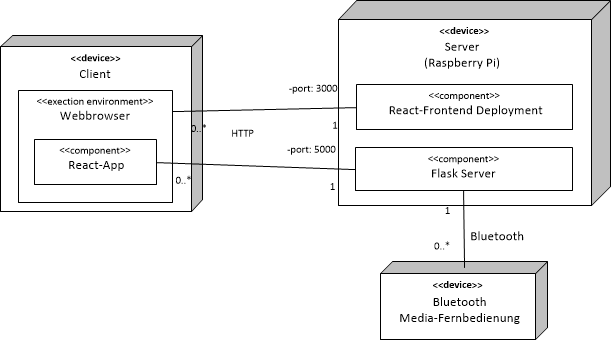
\includegraphics[width=\textwidth]{Bilder/Verteilungssicht.png}\\
	\captionof{figure}{Verteilungs-Diagramm}
	\label{fig:verteilusgssicht}
\end{minipage}
\\
\\
\\
Als Server wird ein Raspberry Pi 3 verwendet, da dieser bei ausreichend Rechenleistung eine Leistungsaufnahme von unter 9 Watt besitzt. Durchschnittlich ist damit zu Rechnen das der Raspberry Pi nicht mehr als 1,5 A verbraucht. Somit kann er mit einer handelsüblichen 5000mAh Powerbank über einen Zeitraum von über 3 Stunden autark betrieben werden. \\
Im Raspberry Pi 3 sind die benötigten Schnittstellen Bluetooth, WLAN und LAN integriert. Somit werden keine zusätzlichen Adapter benötigt.\\
Als Betriebssystem wird Ubuntu Server 20.4.1 verwendet.\\
Um das System komplett autark verwenden werden kann, hosted der Raspberry Pi einen ad-hoc Access-Point. Dazu werden die Programme \glqq hostapd\grqq{} und \glqq isc-dhcp-server\grqq{} verwendet. Außerdem wird an Stelle des von Ubuntu vorinstallierten Network-Manager die von Debian bekannte Konfiguration über die interfaces Datei verwendet.\\
\\
Ein Client-Gerät kann für die autarke Nutzung über die SSID "Matchcouter" mit diesem Access-Point verbunden werden. Alternativ kann der Raspberry Pi über LAN mit einem bestehendem Netzwerk verbunden werden, damit alle Geräte dieses Netzwerks als "Display" verwendet werden können. \\
Auf den Client-Geräten muss im Webbrowser Port 3000 des Raspberry Pis aufgerufen werden um das Frontend zu erhalten. Das Frontend kommuniziert anschließend über den Port 5000 mit dem Flask-Server.\\
\\
Zur Steuerung werden eine oder mehrere Media-Fernbedienungen von PEARL genutzt. Diese müssen manuell mit dem Raspberry Pi gekoppelt werden und melden sich als \glqq human interface device\grqq{} .
             